\chapter{A Crítica Comportamentalista}
\label{cap:comportamental}

Os grandes pioneiros do estudo das finanças comportamentais foram os pesquisadores
Daniel Kahneman e Amos Tversky. Ambos foram co-autores de diversos trabalhos na área, que
incentivaram o aprofundamento do estudo da psicologia dentro da alocação de recursos na
economia.

Os primeiros trabalhos surgiram na década de 70, tentando modelar o comportamento dos investidores e quais eram as principais armadilhas psicológicas que afetavam a tomada de decisão. Dentre os principais pontos levantados pelos pesquisadores, estão:

\begin{itemize}
	\item Heurísticas de representatividade
	\item Disponibilidade
	\item Efeito ancoragem
\end{itemize}
 
Para Kahneman e Tversky, os investidores sofrem do problema de representatividade. Isto significa que, para estimar cenários de probabilidade, normalmente são utilizadas heurísticas na tomada da decisão, que acabam desviando da real representação desejada. Heurísticas são
fatores simplificadores de pensamento: formas de padronizar e estereotipar comportamentos para facilitação da compreensão.

A disponibilidade é um conceito que trata sobre como informações recentes influenciam no julgamento das probabilidades e predições. Desta forma, são gerados vieses que deslocam a análise do real valor. É um ponto importante que fundamentou a pesquisa de inúmeros comportamentalistas, como Werner F. M. De Bondt e Richard Thaler, que trataram da hipótese das reações exageradas e que é o próximo conteúdo a ser comentado no trabalho.

Kahneman e Tversky também descobriram o chamado efeito ancoragem,  em que tomadores de decisão são influenciados por uma “base” ou “valor inicial”; ou seja, também é possível criar vieses a partir de valores e informações que fogem da ideia fundamental. Desta forma, ambos os pesquisadores solidificaram a introdução do comportamento humano afetando a tomada de decisão na alocação de recursos, abrindo caminho para ideias complementares na hipótese dos mercados eficientes.

\section{Hipótese das reações exageradas}

\citeonline{Bondt1985}, descobriram que os preços das ações reagem de forma exagerada, evidenciando características de um mercado fracamente eficiente. Este documento marcou o início das finanças comportamentais.

Ambos defendem a ideia de que os agentes econômicos dão um peso maior para as informações mais recentes, fazendo com que flutuações diárias tenham grande influência na tomada de decisão dos gestores. Esta ideia é fortalecida por \citeonline{Shiller1981}, que defende que as flutuações dos mercados não são compatíveis com a incidência de pagamento de dividendos. Ou seja, os movimentos nos preços não são racionais pois fogem do real valor dos ativos, que deriva da reação exagerada dos agentes em relação aos acontecimentos. Assim, “investidores têm a tendência de dar uma importância desproporcional a eventos econômicos de curto prazo”.

Assim, um questionamento surge: quais são as condições de equilíbrio para mercados no qual alguns agentes não possuem comportamento racional, no sentido de não revisar as suas expectativas? Para isso, Bondt e Thaler desenvolveram alguns testes empíricos para tal. No caso de uma mudança súbita nos preços de ativos do mercado acionário, Bondt e Thaler chegaram a duas hipóteses: 

\begin{itemize}
	\item Movimentos extremos nos preços vão ser seguidos por uma por um movimento contrário ao do choque; 
	\item Quanto maior for o choque nos preços, maior será o ajuste seguinte.
\end{itemize}

Ambas hipóteses violam a forma fraca de eficiência de mercado. Assim, os pesquisadores tiveram o objetivo de testar se as hipóteses de reações exageradas em flutuações de curto prazo são previsíveis. Para isso, Bondt e Thaler separaram portfólios de ações em duas categorias: os “vencedores” e os “perdedores”.

Tendo os retornos acumulados de várias ações, eles formaram portfólios com ações que obtiveram retornos entre os 10\% melhores (quantil 90\%), que foram classificados como os vencedores, e os portfólios que ficaram ações com retornos entre os 10\% piores (quantil 10\%) foram classificados como os perdedores. Assim, como foi o comportamento visto no retorno destes portfólios montados nos meses seguintes? Bondt e Thaler usaram a abordagem do CAR (cumulative average residual).

\begin{figure}[h]
	\centering
	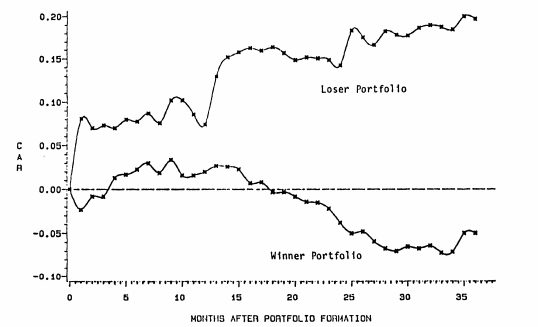
\includegraphics[width=1\linewidth]{figs/fig_comp_winner}
	\caption[Retornos de portfólios vencedores e perdedores]{Retornos residuais de portfólios formados com ações vencedoras e perdedoras.\\ Fonte: \citeonline{Bondt1985}}
	\label{fig:figcompwinner}
\end{figure}

Os resultados dos testes se encaixaram na teoria da hipótese de reações exageradas. Portfólios com ações do quantil 10\% performaram em até 19.6\%, em média dos 36 meses seguintes, que o mercado. Já os portfólios vencedores, do quantil 90\%, performaram em média 5\% abaixo do mercado. Assim, o módulo da diferença entre os portfólios vencedores e perdedores ficou em 24.6\%.

Assim, algumas evidências foram encontradas:

\begin{itemize}
	\item O efeito de reação exagerada é assimétrico: é muito maior para os perdedores que para os vencedores;
	\item Boa parte dos retornos excessivos vêm no mês de janeiro (melhores perspectivas de um novo ano, quem sabe?
\end{itemize}

\section{Estratégias que buscam valor}

\citeonline{Lakonishok1994}, fornecem evidências de que as estratégias de valor geram retornos mais altos porque essas estratégias exploram o comportamento sub-ótimo do investidor típico e não porque estas são fundamentalmente mais arriscadas.Essas estratégias de valor são contrárias às estratégias “ingênuas”, que podem ir desde dar muita importância a retornos passados até ter reações exageradas em relação a notícias más ou boas; assim, obteriam melhores retornos.
Em uma menção a hipótese das reações exageradas, Lakonishok diz que os gestores que “apostam contra” esta visão ingênua obtém melhores retornos pois investem desproporcionalmente em ações que estão subvalorizadas e investem menos em ações supervalorizadas. Assim, seria possível que alguns investidores “batessem o mercado”.

\citeonline{Kahneman1982} explicam que predições intuitivas são, tipicamente, não regressivas: pessoas comumente fazem predições com informações cuja validade preditiva e confiabilidade são questionáveis, como se ancorar em dados passados que tiveram ótimo desempenho (que em algum momento regredirão à média). Assim, investidores poderiam bater os ingênuos vendendo ações que tiveram grande desempenho passado e com grandes expectativas de retorno para o futuro e, do outro lado, comprar ações com baixos retornos passados e com poucas expectativas de retornos para o futuro. Desta forma, é aproveitado o conceito de reversão à média para projeções de retornos.

Tendo os chamados “investidores contrários” obtido melhores retornos ao longo do tempo, surge a pergunta: seriam as suas estratégias mais arriscadas? Seria esse o motivo dos melhores retornos? Duas teorias foram propostas para explicar porque estratégias de valor produziram melhores retornos. A primeira diz que os investidores contrários/de valor exploraram os erros dos investidores ingênuos; a segunda teoria diz que eles poderiam estar mais expostos ao risco.

Para isso, dois conceitos são importantes neste estudo: 

\begin{itemize}
	\item As ações de valor são aquelas com baixo desempenho passado e com pouca esperança de retornos no longo prazo no ponto de vista dos investidores (que já citamos parágrafos acima);
	\item As ações “glamorosas”: são aquelas com alto desempenho passado e com grandes expectativas de retornos para o futuro.
\end{itemize}

\begin{figure}
	\centering
	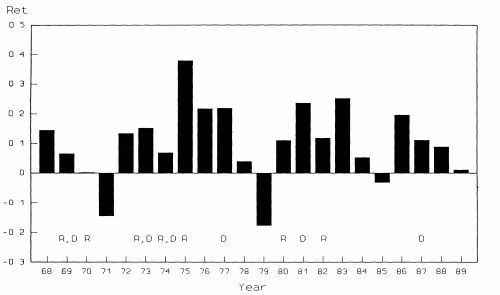
\includegraphics[width=1\linewidth]{figs/fig_comp_value}
	\caption[Retornos de estratégias Valor versus Glamor]{Retornos de estratégias Valor versus Glamor.\\ Fonte: \citeonline{Lakonishok1994}.}
	\label{fig:figcompvalue}
\end{figure}

Na figura \ref{fig:figcompvalue}, vemos a diferença entre os retornos das ações de “valor” e retornos das ações de “glamour”. Em apenas três anos dentre a série estudada esta relação foi negativa, ou seja, com ações glamorosas tendo melhor desempenho. No final, a conclusão foi de que, visto que os dados de crescimento de fluxo de caixa e outros tipos de dados das empresa foram muito menores que o esperado pelo mercado, foi entendido que os agentes superestimaram consistentemente estas “empresas glamorosas”. Uma das propostas foi de que as ações de valor apresentaram maior risco, o que foi desmentido: os indicadores fundamentais de análise de risco mostraram pouca diferença entre as ações de “valor” para as ações “glamour”.

\section{Psicologia, arbitragem e mercado eficientes}

Para \citeonline{Sharpe1990}, o conceito fundamental de arbitragem é de negociações simultâneas de compra e venda de um ativo essencialmente similar ou igual em dois diferentes mercados, ganhando na diferença de preços. Além disso, para \citeonline{Shleifer1997}, a arbitragem tem um papel crucial em levar os preços para o seu valor fundamental e para manter os mercados eficientes. Dada a importância da arbitragem na teoria dos mercados eficientes, como o comportamento dos agentes econômicos afeta o papel da arbitragem?

No modelo de arbitragem implícita de \citeonline{Fama1965}, ele assume a hipótese de um mercado com um número gigantesco de pequenos “arbitradores”, cada um tomando uma posição infinitesimal contra o descolamento de preços do valor fundamental em uma variedade de mercados. Também, como as suas posições são pequenas, falta de capital não é um problema e os arbitradores são neutros em relação ao risco. Assim, na coletividade das ações de todos os agentes, os preços voltariam para o valor fundamental. Porém, para \citeonline{Shleifer1997}, um dos maiores problemas deste modelo é de que geralmente, estes pequenos arbitradores não são os agentes que possuem conhecimento e informação para atuar com arbitragem; geralmente, a arbitragem é conduzida relativamente por pouco profissionais, extremamente especializados.

A crítica de que a arbitragem não é perfeitamente eficiente para levar os mercados à eficiência é a de que os arbitradores podem sofrer da aversão ao risco dos parceiros, aqueles que lhe confiam para gerir os seus investimentos. Ao contrário de arbitradores que utilizam do próprio capital para a alocação de recursos e se baseiam no retorno esperado das negociações, os investidores, por outro lado, podem alocar os seus investimentos baseados no retorno passado dos arbitradores. Assim, em momentos que o arbitrador precisasse de mais recursos por já estar totalmente posicionado, ele não teria esse suporte e, assim, perder as melhores oportunidades de descolamento de preços. Além disso, o acontecimento deste cenário também afeta o comportamento do arbitrador, que ficará mais cauteloso em fazer suas negociações. A conclusão: o arbitrador não conseguirá sempre ter uma ação racional e, com isso, a arbitragem se torna menos eficiente para fazer o mercado alcançar a sua eficiência.

